\section{Quantum Programming}\label{sec:lit_rev:quantum_programming}

The mathematical and physical foundations of quantum computation are assumed throughout; qubits, gates and measurement are established in Chapter~\ref{ch:introduction} and are not revisited here.

This section examines what those foundations are assembled into.
It surveys the abstract models of quantum computation, the programming paradigms constructed over them and the semantic pressures that recur across quantum languages regardless of which model underlies them.
Although the surveyed models are computationally equivalent, programming systems privilege the circuit model almost without exception; the reasons for that dominance and its consequences for language design form a core part of the analysis in this section.
The section is concerned with models of computation and programming paradigms, not with compilation pipelines and intermediate representations; those are examined in Section~\ref{sec:lit_rev:compilation}.

\subsection{Models of Quantum Computation}\label{subsec:lit_rev:quantum_programming:models_of_computation}

Quantum computation can be described through three families of abstract machine models, each addressing a different question about the nature of computation.
Computation-definition models, including the quantum Turing machine and the quantum lambda calculus, provide formal accounts of what quantum computation is~\cite{nunez_corrales2025betterabstractmachines,wang2023qrasp}.
Instruction-execution models, including the quantum random access machine and stored-program variants, specify how it is described and run at the level of an addressable machine~\cite{nunez_corrales2025betterabstractmachines,wang2023qrasp}.
Execution models specify how computation is encoded as a process; they define a computational paradigm rather than a hardware substrate.
The circuit, measurement-based (MBQC), adiabatic, quantum walk, quantum cellular automata (QCA) and ancilla-driven (ADQC) models populate this third family.
Table~\ref{tab:lit_rev:quantum_programming:execution_model_descriptions} describes each model, Figure~\ref{fig:lit_rev:quantum_programming:model_mechanisms} provides a graphical interpretation.

\begin{table}[htbp]
    \centering
    \caption{The execution models of quantum computation and the form each gives a computation.}
    \label{tab:lit_rev:quantum_programming:execution_model_descriptions}
    \footnotesize
    \begin{tabularx}{\textwidth}{@{}lX@{}}
        \toprule
        \textbf{Model} & \textbf{Description} \\
        \midrule
        \textbf{Circuit} & A computation is a sequence of unitary gates applied to quantum registers~\cite{yao1993circuit}. \\
        \textbf{Measurement-based (MBQC)} & A computation proceeds through adaptive single-qubit measurements on a pre-entangled resource state~\cite{raussendorf2001oneway}. \\
        \textbf{Adiabatic} & A solution is encoded in the ground state of a target Hamiltonian, reached by slowly evolving from an initial one~\cite{aharonov2007adiabatic}. \\
        \textbf{Quantum walk} & The states of the system are the vertices of a graph and the edges fix the permitted transitions, so the computation is shaped by the structure of the graph rather than by an explicit sequence of operations~\cite{childs2009quantumwalk}. \\
        \textbf{Quantum cellular automata (QCA)} & A lattice of quantum systems evolves under a single rule applied identically to every site at each step, with no central processor issuing addressed operations; the program is the initial configuration of the lattice~\cite{farrelly2020qca}. \\
        \textbf{Ancilla-driven (ADQC)} & A register is manipulated entirely through a sequence of interactions with a single auxiliary qubit measured after each coupling, with no direct operations on the register~\cite{anders2010ancilladriven}. \\
        \bottomrule
    \end{tabularx}
\end{table}

\begin{figure}[htbp]
    \centering
% ===========================================================================
% F2 -- Mechanism detail per execution model. Four panels (a)-(d).
% Placement: Beat 5. Companion to the comparison table (T3).
%
% ----- intended drawing -----------------------------------------------------
% (a) Circuit -- ordered unitary gates on wires, time runs left to right
%
%     |0> --[H]--*--------[M]
%                |
%     |0> -------(+)--[H]-[M]
%        (control-dot on top wire, target (+) on bottom; M = measurement)
%
% (b) Measurement-based -- a 2-row lattice of qubits joined into a
%     pre-entangled resource state; qubits measured left to right
%
%     o -- o -- o -- o
%     |    |    |    |
%     o -- o -- o -- o
%        ==> measurement sweep (order 1,2,3,4 ...)
%
% (c) Adiabatic -- two energy levels vs interpolation parameter s in [0,1];
%     an avoided crossing near s ~ 0.5 marks the minimum spectral gap
%
%     E |  \                    /   E1(s)  (dashed, upper branch)
%       |   \__              __/
%       |      \____ Dmin ___/        <-- minimum gap at the avoided crossing
%       |      ____/      \____
%       |  ___/                \___   E0(s)  (solid, lower branch)
%       +----------------------------- s
%       0                            1
%     (annotate the vertical gap between branches as \Delta_{min})
%
% (d) Quantum walk -- scattering widget on a graph; a walker enters on an
%     input rail, scatters through the gadget, leaves on an output rail
%
%     input rail >--o--o--[ WIDGET subgraph ]--o--o--> output rail
%                              (effects the gate)
%     arrow shows traversal direction = the order in which the computation runs
%
% NOTE on (d): redraw the scattering-gate gadget from childs2009quantumwalk
%   (source figure is in the childs note); do NOT invent its topology.
% ---------------------------------------------------------------------------
    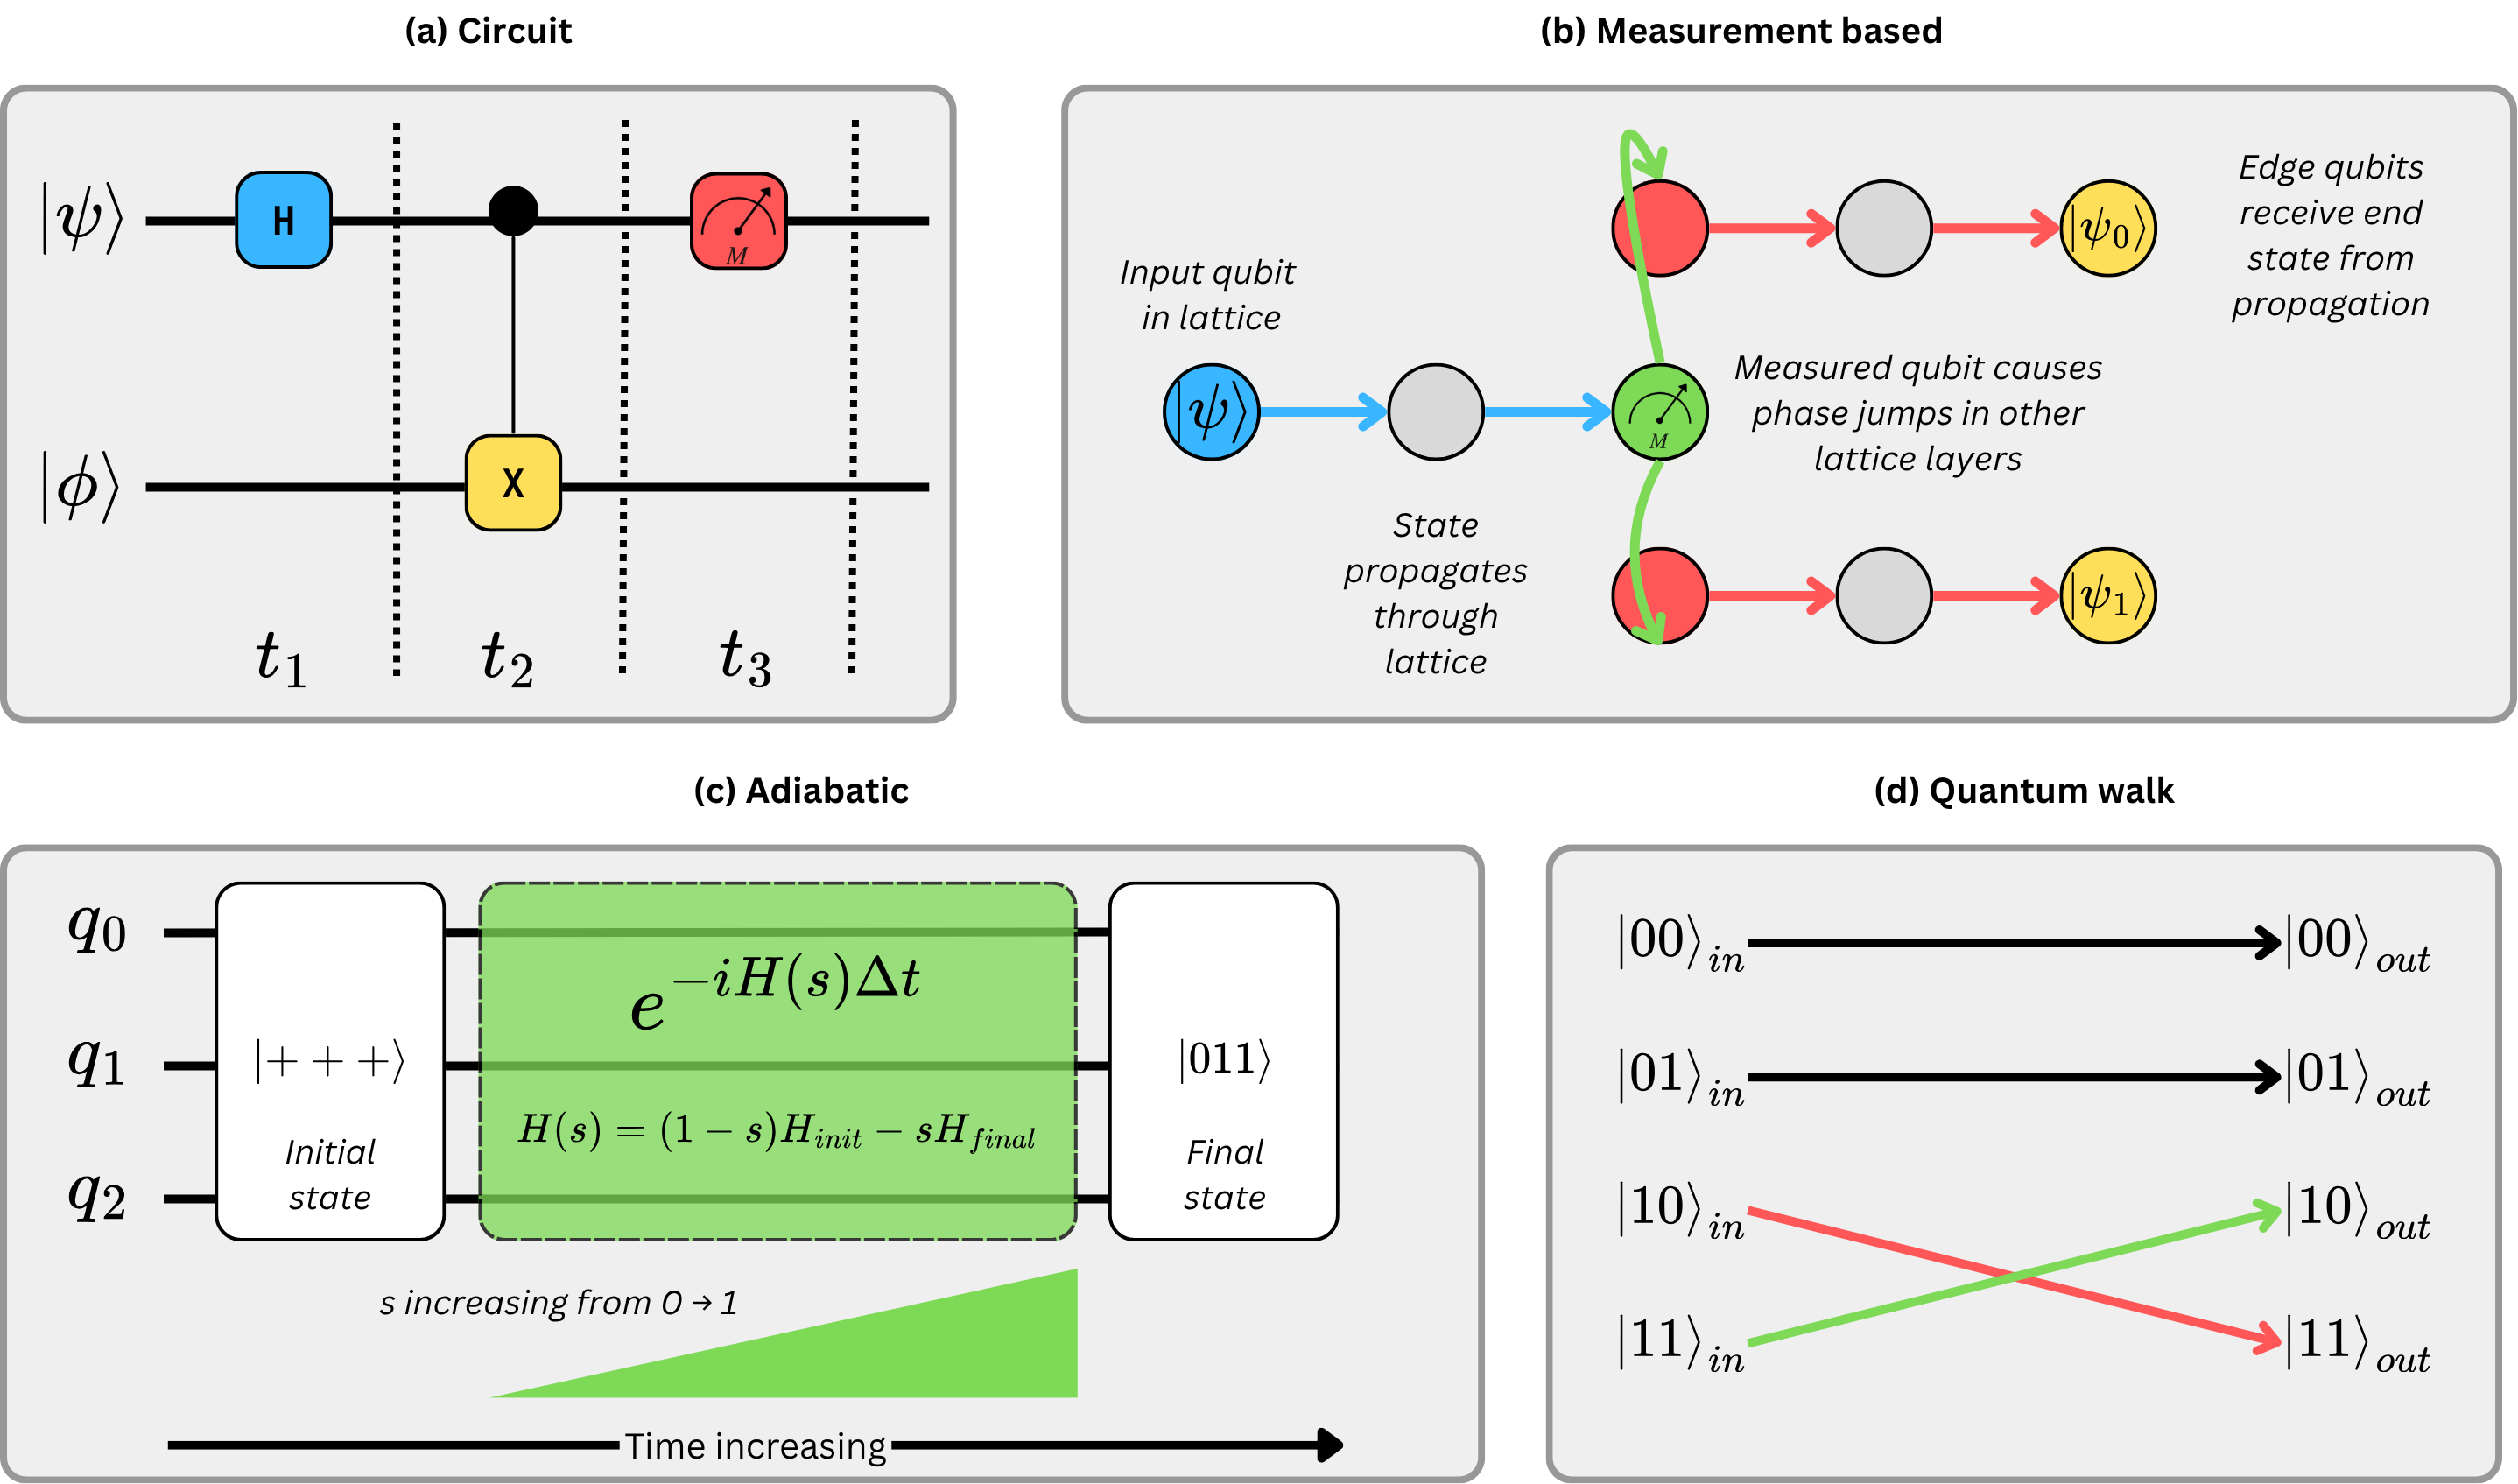
\includegraphics[width=\textwidth]{../figures/fig-lit_rev-quantum_programming-model_mechanisms}
    \caption{The mechanism each execution model uses to carry a computation: (a) the circuit composes ordered unitary gates (b) the measurement-based model drives adaptive measurements across a pre-entangled resource state (c) the adiabatic model relies on the minimum spectral gap that bounds its evolution (b) the quantum walk routes a walker through a scattering widget.}
    \label{fig:lit_rev:quantum_programming:model_mechanisms}
\end{figure}

All three families achieve universal quantum computation and the execution models are polynomially equivalent to one another~\cite{aharonov2007adiabatic,childs2009quantumwalk,farrelly2020qca}.
They differ not in computational power but in what each encodes into the structure of a well-formed program: the circuit model requires explicit specification of every gate and qubit.
MBQC encodes computation in a resource state and a measurement pattern; QCA encodes it in an initial lattice configuration under a fixed rule.
These differences are not incidental to language design; a programming language built on a given model inherits its structural assumptions and can only hide from the programmer what the model itself makes implicit.

Computation-definition models provide a formal account of what quantum computation is, independent of how a program is described or run.
The quantum Turing machine is the canonical model of this kind, generalising the classical Turing machine so that the transition function assigns a complex amplitude to each move~\cite{bernstein1997quantum}.
Its evolution is required to be unitary.
Where a probabilistic Turing machine keeps its move probabilities summing to one, the quantum machine must evolve so that the squared amplitudes across all configurations continue to sum to one.
This ensures the machine is in a physically realisable state at every step and guaranteeing that measurement yields a genuine outcome~\cite{bernstein1997quantum}.
Reversibility follows from this requirement rather than being imposed separately, and definite outcomes arise only when the final superposition is measured~\cite{bernstein1997quantum}.
The quantum lambda calculus reaches an equivalent account through a higher-order, type-theoretic route, characterising quantum computation in terms of functions rather than machine configurations~\cite{nunez_corrales2025betterabstractmachines}.

Well-formedness in these models is a global semantic property rather than a syntactic one.
In the quantum Turing machine, a transition function is legal precisely when the operator it induces over the space of configurations is unitary, a condition that no local rule of grammar can enforce on its own~\cite{bernstein1997quantum}.
This is a constraint on quantum computation itself rather than on any particular machine~\cite{bernstein1997quantum}; the reversibility it imposes is inherited by every execution model and every language constructed above them.
These models therefore fix what a quantum program must satisfy without prescribing how it is encoded or executed, establishing the model-invariant discipline against which the structural commitments of the execution models can be assessed.

Instruction-execution models describe how a quantum program is expressed as a sequence of operations and run on an addressable machine.
The quantum random access machine pairs a classical controller with a quantum register and exposes only three operations on that register: preparing a state, applying a unitary and measuring~\cite{knill1996pseudocode}.
A quantum register is treated as a classical register not known to hold a classical value, so the line between classical and quantum data is drawn by the operations permitted rather than by the storage itself~\cite{knill1996pseudocode}.
Control remains entirely classical, with the controller issuing unitaries and reading results back through measurement while reusing familiar constructs such as assignment and conditional execution~\cite{knill1996pseudocode}.
A formal development of the model adds a finite instruction set over unbounded classical and quantum registers.
Its stored-program variant places the program in those registers with an instruction counter, allowing the machine to modify its own instructions as it runs~\cite{wang2023qrasp}.
Both machines simulate and are simulated by the quantum Turing machine within polynomial time bounds, adding an apparatus for describing and running programs without changing what can be computed~\cite{wang2023qrasp}.
Figure~\ref{fig:lit_rev:quantum_programming:instruction_execution} demonstrates this pattern.

\begin{figure}[htbp]
    \centering
% ===========================================================================
% F4 -- Instruction-execution architecture and the fetch--execute cycle.
% Placement: Beat 3 (instruction-execution family: QRAM, QRASP, QRM, QCM).
% Intent: a classical control layer sits between a stored program and the
%   quantum register; measurement results return to the classical state and
%   select the next instruction (the "classical scaffold" of the prose).
%
% ----- intended drawing -----------------------------------------------------
% (a) Architecture
%
%     [Program counter] ---- address ----> [Instruction memory]
%            ^                                      |
%            |                                  instruction
%          branch                                  v
%            |                                  [ Decoder ]
%            |                                      |
%            |                                   gate / op
%            |                                      v
%     [Classical registers] <-- measurement -- [Quantum register]
%
% (b) Fetch--execute cycle (clockwise loop)
%
%        Fetch  ----------->  Decode
%          ^                     |
%          |                     v
%        Measure/update  <----  Execute
%
% Notes: solid arrows = data/control flow; the branch arrow closes the loop
%   from classical registers back to the program counter; shade the quantum
%   register box to distinguish it from classical components.
% ---------------------------------------------------------------------------
    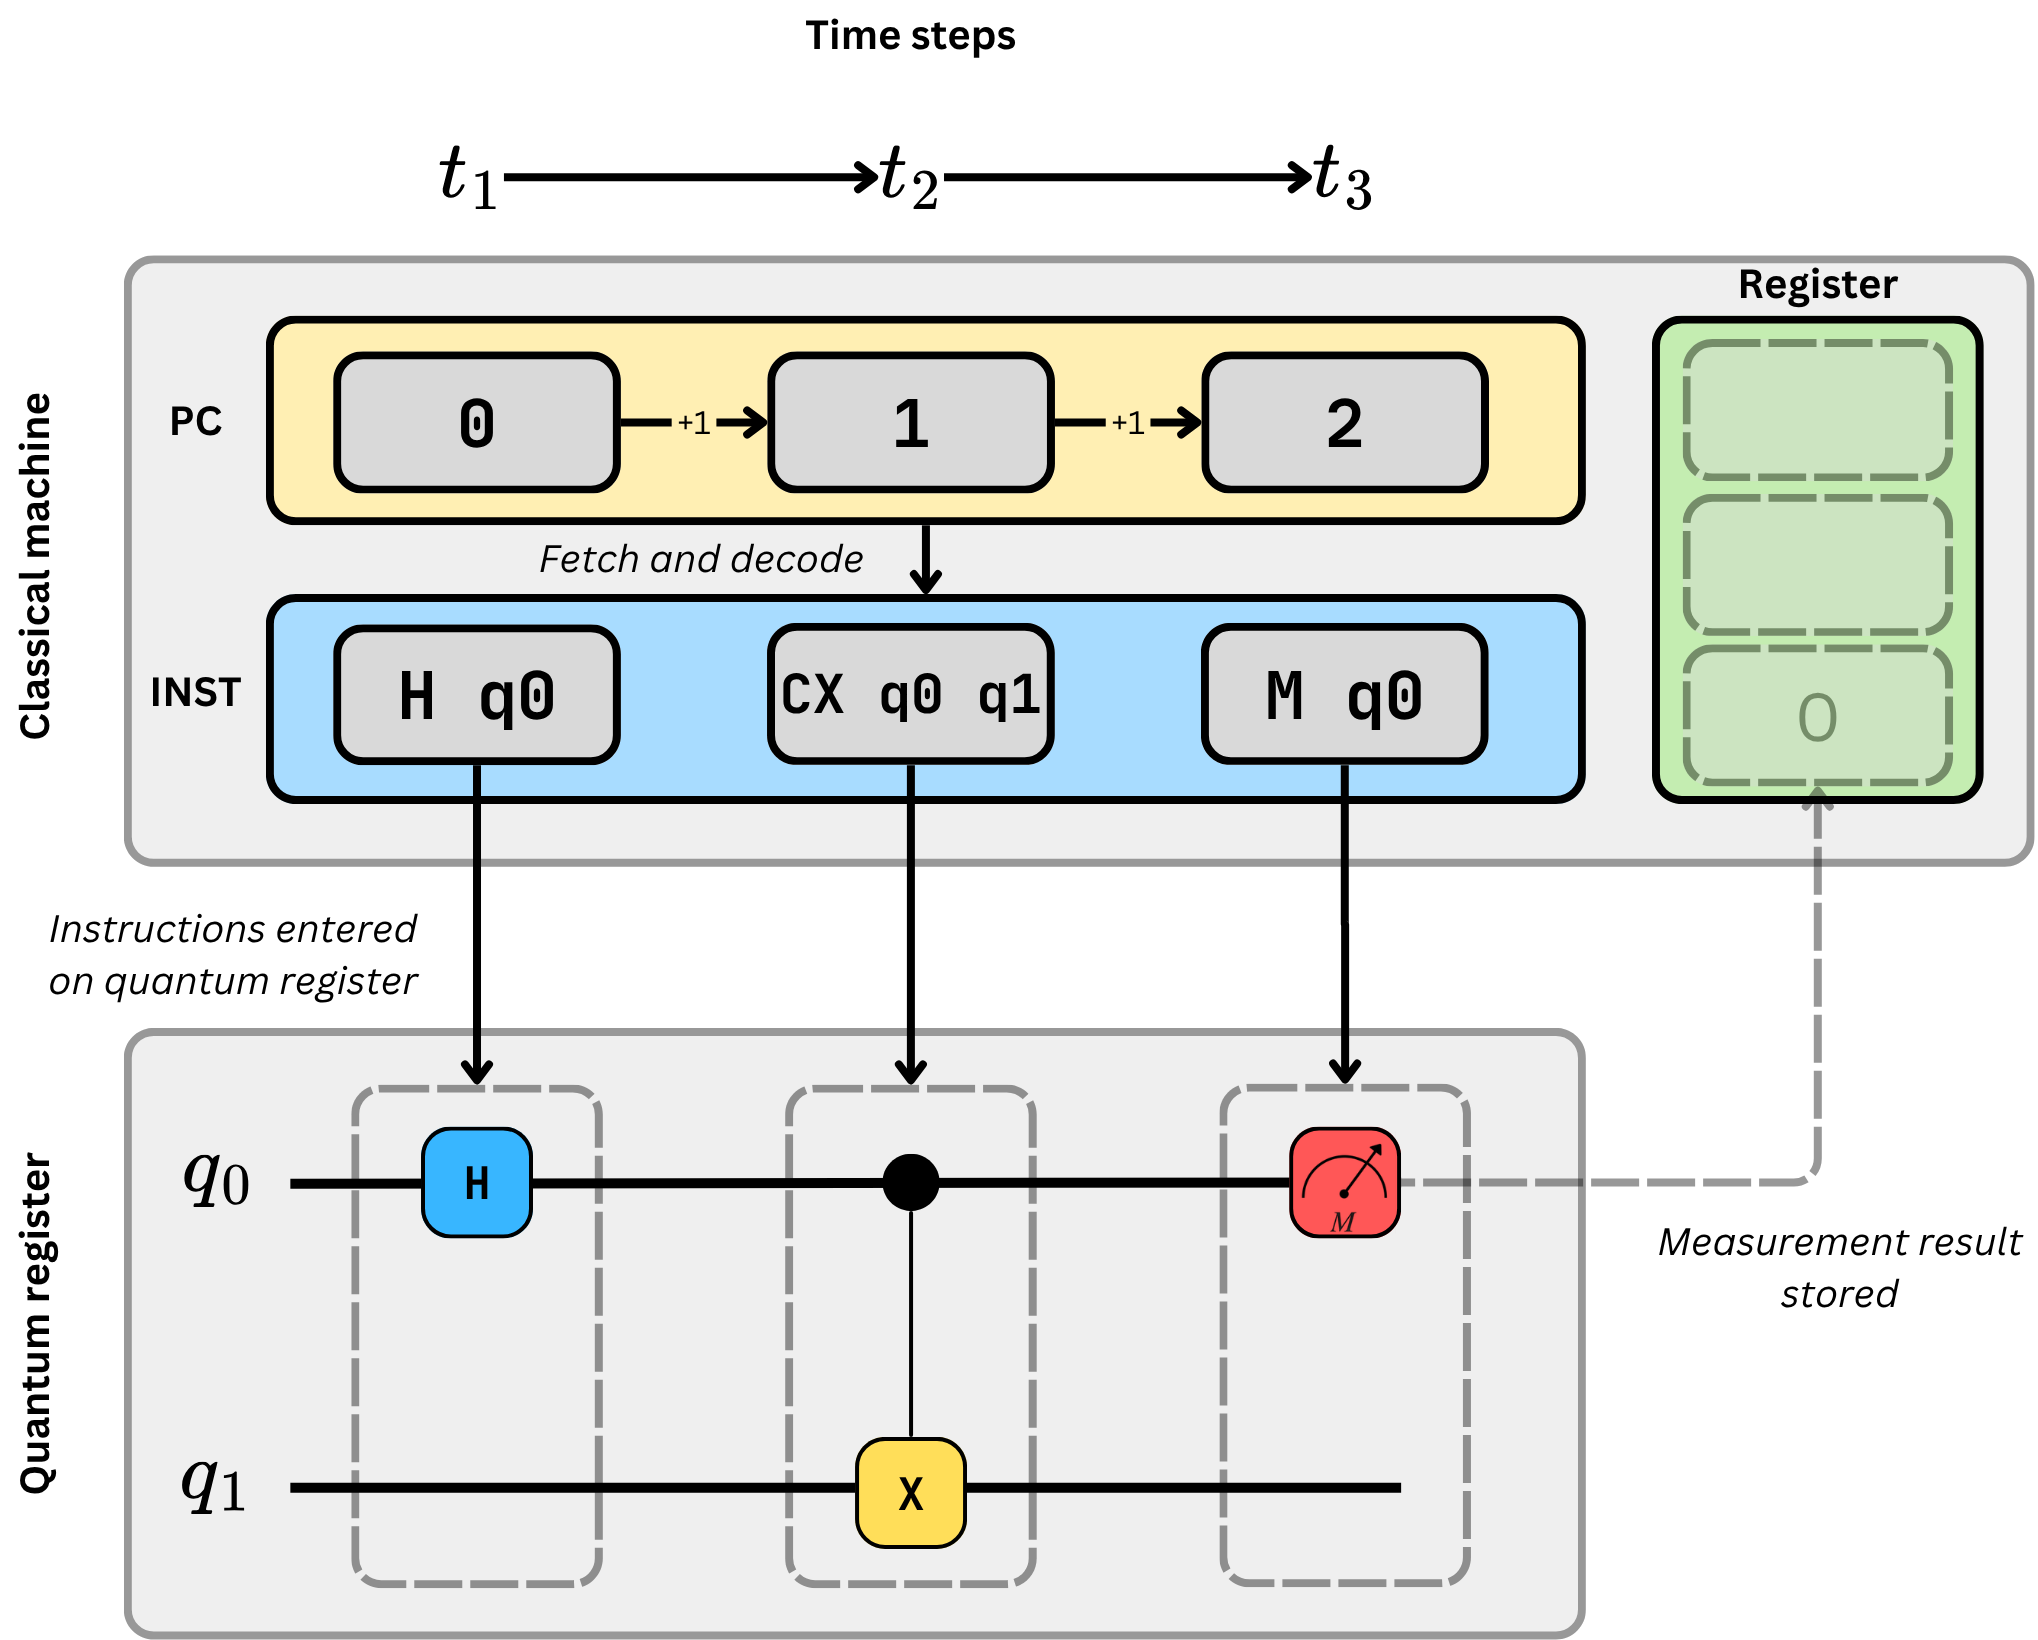
\includegraphics[width=\textwidth]{../figures/fig-lit_rev-quantum_programming-instruction_execution}
    \caption{A diagram displaying the use of a classical control register for program execution in models such as QRAM and QRASP.}
    \label{fig:lit_rev:quantum_programming:instruction_execution}=
\end{figure}

The structural commitments of these models become visible where control itself is made quantum rather than left to a classical controller.
The quantum control machine replaces the classical instruction cycle with one in which fetching, executing and retiring each instruction are unitary operations over quantum control registers, the program counter among them~\cite{yuan2025foundationalabstractions}.
A classical conditional jump overwrites the program counter and discards which branch was taken, an operation that is not injective and so cannot be realised as a unitary~\cite{yuan2025foundationalabstractions}.
In superposition this irreversibility entangles the control state with the data and cancels the interference the computation depends on, so a direct lift of classical control flow is physically impossible rather than merely inefficient~\cite{yuan2025foundationalabstractions}.
Realisable control flow must therefore be injective, retaining enough history to stay reversible, and synchronised, so that every branch of a superposition reaches the same program point at the same step; bounded loops are the only quantum loops these conditions admit~\cite{yuan2025foundationalabstractions}.
The unitarity discipline fixed by the computation-definition models thus propagates upward into the instruction set, governing which control constructs an execution model may even offer.

The criteria for a productive quantum abstract machine were established in the assessment of abstraction in Section~\ref{sec:lit_rev:abstraction}, where the conclusion was that no existing machine satisfies the full set and that the requirements for a symbolic instruction architecture are the principal gaps~\cite{nunez_corrales2025betterabstractmachines}.
Those conclusions can be tested against the three families described above.
The criteria apply unevenly, since several of them presuppose a model that already claims to be a programmable machine.
The computation-definition models fix what a computation is and provide no instruction set, so the demand for a stable and hardware-independent architecture falls on the instruction-execution family rather than on them.
The quantum random access and stored-program machines in that family are judged to fail the requirement that machine state be finite and addressable in advance,on the grounds that they assume unbounded registers~\cite{nunez_corrales2025betterabstractmachines}.
This judgement is too strong.
A stored-program machine occupies only finitely many registers at any step, and a time-constructible program can compute its own resource bound from its input with certainty, fixing that bound before it runs~\cite{wang2023qrasp}.
An unbounded register file is in any case the same idealisation made by the classical random access machine, which the same criteria hold up as a model of effective abstraction~\cite{nunez_corrales2025betterabstractmachines}.
The requirement that excludes the quantum machines on this basis is better read as a demand for addressable and decomposable state, which the stored-program machine provides.

A second criterion, that instructions be symbolic rather than tied to circuit elements, is met only in part.
The control and memory instructions of these machines, among them load, store, branch and arithmetic, abstract over their realisation much as an addition instruction stands apart from any particular adder~\cite{wang2023qrasp}.
Their quantum instructions do not.
An instruction to apply a Hadamard or Pauli operator names a gate of the circuit model, and its meaning is the amplitude transformation that gate performs rather than a higher account of the operation being carried out~\cite{nunez_corrales2025betterabstractmachines}.
The separation between instruction symbol and circuit element that the classical instructions achieve is absent for the quantum ones, and this, rather than any wholesale dependence on circuits, is what keeps the models reasoning in circuit terms~\cite{nunez_corrales2025betterabstractmachines}.

The criteria also separate classical control flow from quantum and hybrid control flow, and requiring a single model to provide both exposes a genuine difference between the families.
The quantum Turing machine has no native control construct.
A fixed transition rule drives its evolution, and the only choice exercised over the computation is the external decision of when to measure~\cite{bernstein1997quantum}.
Its control is classical only by omission, residing outside the quantum state rather than being expressed within the machine.
The quantum control machine takes the opposite approach, placing the program counter and a branch register into the quantum state so that branching itself can occur in superposition~\cite{yuan2025foundationalabstractions}.
This does not make its control non-classical.
The machine runs a classical instruction cycle and admits only loops whose length is fixed in advance.
It requires that the separate branches of a superposition be brought back into agreement before the program ends, so that the control registers hold a single definite value at termination and the running time does not depend on any quantum variable~\cite{yuan2025foundationalabstractions}.
This last condition, termed synchronisation, is what allows superposed control to remain classically well-behaved at the points where the program begins and ends~\cite{yuan2025foundationalabstractions}.
Quantum control flow is therefore layered on a classical control structure rather than replacing it.
The model that comes closest to providing both forms of control does so not by preferring one to the other but by running quantum control within a classical scaffold.
Its remaining shortfalls lie in the abstraction of its instructions and in its physical realisability rather than in any failure to combine the two~\cite{yuan2025foundationalabstractions, nunez_corrales2025betterabstractmachines}.

The execution models describe how a computation is encoded as a physical process rather than what it computes or how its instructions are sequenced.
The circuit model composes a computation from elementary gates~\cite{yao1993circuit}, the measurement-based model drives it through adaptive measurements on a pre-prepared entangled state~\cite{raussendorf2001oneway}.
The adiabatic model holds the answer in the ground state of a slowly varying Hamiltonian~\cite{aharonov2007adiabatic} and the quantum walk model encodes it in the dynamics of a walker over a graph~\cite{childs2009quantumwalk}.
Each simulates and is simulated by the circuit model within polynomial bounds, so all four characterise the same class of efficiently solvable problems.
Equivalence of this kind settles the question of power; it leaves untouched the question of representation, of how readily a model lets a computation be expressed and reasoned about.
The models are equivalent in power and differ only in how each realises sequencing, the role played by time, and it is this difference that governs how readily each can be expressed, as set out in Table~\ref{tab:lit_rev:quantum_programming:execution_models}.

\begin{table}[htbp]
    \centering
    \caption{Comparison of execution models by what realises the order of its operations, the trade-off between the physical advantage it offers and the complexity this imposes on representation.}
    \label{tab:lit_rev:quantum_programming:execution_models}
    \footnotesize
    \begin{tabularx}{\textwidth}{@{}lXX@{}}
        \toprule
        \textbf{Model} & \textbf{Sequencing realised by} & \textbf{Representational trade-off} \\
        \midrule
        \textbf{Circuit} & An explicit sequence of gates fixes the order of operations & It is the direct baseline, with gates mapping straight onto operations, but it is  strictly sequential, so circuit depth and gate count grow at least linearly with the computation. \\
        \textbf{Measurement-based (MBQC)} & The order of the adaptive measurements fixes the order of operations & Entanglement is prepared in advance and only one class of operation is required, but the corrections this introduces propagate across the pre-entangled resource state and must be tracked non-locally by classical feed-forward. \\
        \textbf{Adiabatic} & A spatial clock register stands in for the passage of time & A spectral gap suppresses leakage from the ground state and protects the computation, but correctness becomes a global property of that gap, which narrows polynomially as the computation lengthens and slows the evolution. \\
        \textbf{Quantum walk} & Traversal from a start vertex to a terminal vertex fixes the order of operations & The graph is low-degree and unweighted, but the computation is carried in global interference and each traversal succeeds only probabilistically, so it must be repeated until success. \\
        \bottomrule
    \end{tabularx}
\end{table}

On that axis the circuit model is the one whose structure coincides with sequential composition.
Its gates carry fixed and context-independent meanings whose composition is the meaning of the whole, a compositionality the other models recover only under a momentum condition, disrupt with tracked corrections, or replace with a global spectral-gap condition~\cite{childs2009quantumwalk,raussendorf2001oneway,aharonov2007adiabatic}.
Its sequencing is already an explicit ordering of operations, the form a program takes, whereas the other models realise time in ways that must be translated back into an ordering to be read or compiled.
Universality for each of the other models is in turn established by reproducing circuits, so the circuit model is already the common form against which the others are defined.

That the circuit model is the most readily expressed is therefore a fact about the programmer's surface rather than about computational power or physical convenience.
The measurement-based and adiabatic models hold physical advantages in resource preparation and in error suppression that the circuit model lacks~\cite{raussendorf2001oneway, aharonov2007adiabatic}.
Its dominance both mirrors and inverts the classical history that motivates the criteria for a good abstract machine.
Classical circuits were expressively complete yet unusable until an instruction set supplied composable operations matching the way programmers reason~\cite{nunez_corrales2025betterabstractmachines}.
Quantum computation has instead adopted the circuit model as its default surface.
A contingent coincidence between one model and the structure of sequential composition thereby hardens into the assumption that time is a gate sequence.
That assumption ascends into intermediate representations and compilers and forces the other models to be implemented as conversions from circuits rather than from their own principles~\cite{aharonov2007adiabatic}.
The models of computation settle what can be computed without settling how a computation should be expressed to the programmer, which is the work of a programming paradigm rather than a computation model.